\documentclass[reqno]{amsart}

\usepackage{External/takodachi}

\renewcommand{\div}{\operatorname{div}}
\newcommand{\nlin}{\mathrm{nlin}}
\newcommand{\lin}{\mathrm{lin}}

\title
{
	Regularity for $L^\infty_t L^3_x$-solutions to Navier-Stokes via rigidity
} 
\author{Jason Zhao}
\date{\today}


\begin{document}
\maketitle

\begin{abstract}
	We give two proofs of the regularity for solutions to the incompressible Navier-Stokes equations which are a priori bounded in the critical space $L^3_x (\mathbb R^3)$, following the concentration compactness method as in Gallagher-Koch-Planchon and the stacking argument of Tao. The overarching idea one should take away is that rigidity arises from unique continuation in the context of Navier-Stokes. 
\end{abstract}

\tableofcontents

\section{Introduction}
Before getting into any multi-linear algebra, it is important to get a grasp of coordinates in linear algebra and how these coordinates respond to change of bases. Let $V$ be an $n$-dimensional real vector space, and denote $V^*$ its dual space. Given a basis $\{e_i\}_i \subseteq V$, there exists a dual basis $\{\epsilon^j\}_j \subseteq V^*$ satisfying 
	\[ \langle e_i, \epsilon^j \rangle = \delta^j_i. \]
Choose another basis $\{\widetilde e_i\}_i \subseteq V$ and denote its dual basis by $\{\widetilde \epsilon^j\}_j \subseteq V^*$. There exists a change of basis matrix $C^k_i \in \mathsf{GL} (\R^n)$ sending the original basis to the new basis,
	\[ \widetilde e_i = C^k_i e_k. \]	
On the other hand, the inverse change of basis matrix $(C^{-1})^j_k \in \mathsf{GL} (\R^n)$, i.e. $(C^{-1})^j_k C^k_i = \delta^j_i$, transforms the original dual basis to the new dual basis 	
	\[ \widetilde \epsilon^j = (C^{-1})^j_k \epsilon^k. \]
Throughout these notes, we will use these \emph{Einstein summation notation}, where repeated indices are summed over, e.g. $a^i b_i := \sum_i a^i b_i$.


\subsection{{Contravariance}}

We say an object is \emph{contravariant} if the coordinate representation \textit{contra-varies} with respect to change of basis, that is, transforms by the inverse matrix $(C^{-1})^j_i$. Such coordinates are indexed by \textit{upper indices}. The prototypical example of a contravariant object is a \emph{vector} $v \in V$. Every vector admits a unique coordinate representation $\{v^i\}_i \subseteq \R$ with respect to the basis $\{e_i\}_i$, i.e.
	\[ v = v^i e_i . \]
Let $\{ \widetilde v^j \}_j \subseteq \R$ be the unique coordinates with respect to the basis $\{\widetilde e_j\}_j$, then the change of coordinates from $\{v^i\}_i$ to $\{\widetilde v^j\}_j$ is given by the inverse change of basis matrix,
	\[ \widetilde v^j = {(C^{-1})}^j_i v^i. \]
Indeed, 	
	\[ v = \widetilde v^j \widetilde e_j  = \left( {(C^{-1})}^j_i v^i \right) \left( C^k_j e_k \right) = \delta^k_i v^i e_k = v^i e_i . \]
We can interpret a choice of basis $\{e_i\}_i$ as endowing $V$ with a ``measuring tool'', where the coordinates $\{v^i\}_i$ representing the resulting ``measurement''. A change of basis corresponds to changing the choice of ``measuring tool'', e.g. we can view a change of basis $\widetilde e_i = \tfrac{1}{100} e_i$ as changing from ``meters'' $e_i$ to ``centimeters'' $\widetilde e_i$, so the corresponding change of coordinates is 
	\[ \widetilde v^i \text{ meters } = 100 v^i \text{ centimeters}. \]




\subsection{Covariance}

We say that an object is \emph{covariant} if the coordinate representation \textit{co-varies} with respect to change of basis, that is, transforms by the matrix $C^k_i$.  Such coordinates are indexed by \textit{lower indices}. The prototypical example of a covariant object is a \emph{covector} $\omega \in V^*$. Every covector admits a unique coordinate representation $\{\omega_i \}_i \subseteq \R$ with respect to the basis $\{\epsilon^i\}_i$, i.e.
	\[ \omega = \omega_i \epsilon^i = \widetilde \omega_j \widetilde \epsilon^j. \]
Let $\{\widetilde \omega_j \}_j \subseteq \R$ be the unique coordinates with respect to the basis $\{\widetilde \epsilon^j\}_j$, then the change of coordinates from $\{\omega_i\}_i$ to $\{\widetilde \omega_j\}_j$ is given by the change of basis matrix,
	\[ \widetilde \omega_j = C^i_j \omega_i \]
Indeed, 
	\[ \omega = \widetilde \omega_j \widetilde \epsilon^j = \left( C^i_j \omega_i \right) \left( (C^{-1})_k^j \epsilon^k \right) =  \delta^i_k \omega_i \epsilon^k = \omega_i \epsilon^i. \]
Scalars are regarded as ``dimensionless'' quantities, so since a covector acting on a vector produces a scalar, they have inverse dimensions. For example, we can view a change of basis $\widetilde \epsilon^j = 100 \epsilon^j$ as changing from  ``meters$^{-1}$'' $\epsilon^j$ to ``centimeters$^{-1}$'' $\widetilde \epsilon^j$, so the corresponding change of coordinates is 
	\[ \widetilde \omega_j \text{ meters$^{-1}$} = \frac{1}{100} \omega_j  \text{ centimeters$^{-1}$}. \]



\section{Concentration compactness}\label{sec:cc}


\begin{proposition}
	There exists a constant $\epsilon_0 > 0$ such that for every sequence $\{\phi_n\}_n$ of solutions to the defocusing \eqref{NLW} on $(-2, 2) \times 4B$ with uniformly small energy
		\begin{align}
			\cE_{\{0\} \times 4B} [\phi_n] 
				&\ll \epsilon_0^2, 
		\end{align}
	and is asymptotically stationary, 
		\begin{align}
			\iint_{(-2, 2) \times 4B} |(Y + b) \phi_n|^2 \, dx \overset{n \to \infty}{\longrightarrow} 0,
		\end{align}
	for some uniformly time-like vector field $Y$ and a smooth function $b$, then, after passing to a subsequence, we can extract a solution $\Phi \in H^{3/2}_{t, x} ((-1, 1) \times B)$ to the defocusing \eqref{NLW} to which the sequence converges strongly in $H^1 ((-1, 1) \times B)$ and 
		\begin{equation}
			(Y + b) \Phi = 0. 
		\end{equation}
		
\end{proposition} 
	
\begin{proof}
	
\end{proof}	


\section{Rigidity}\label{sec:rigid}
Our goal now is to show that, in view of its compactness, our minimal blow-up solution cannot exist, completing the proof of Theorem \ref{thm:ESS}. We cite \cite{KenigKoch2011}. The strategy can be summarised by the following figure:


\begin{figure}[h]
	\begin{center}
		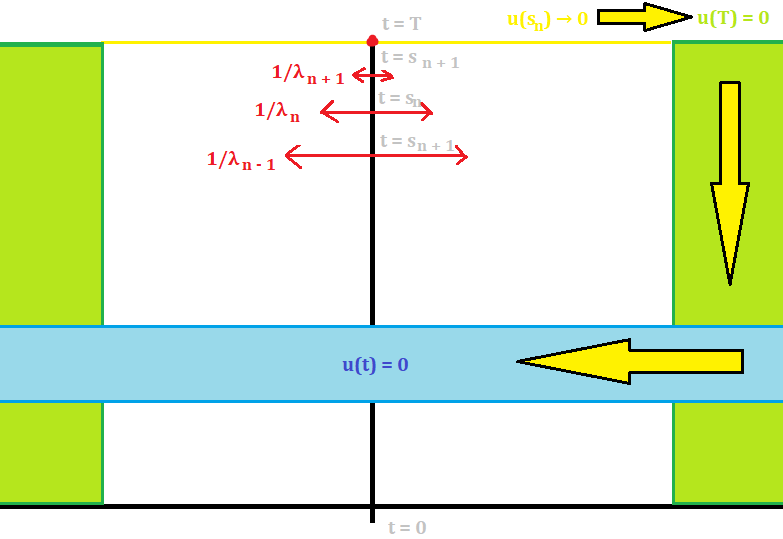
\includegraphics[scale = 0.7]{graphics/rigidity}
		\caption{By compactness, minimal blow-up solutions cannot have any radiation, i.e. $u_{\mathrm{crit}}(t) \rightharpoonup 0$ as $t \to T^*$, since it concentrates into small scales $1/\lambda_n \to 0$. We know $u_{\mathrm{crit}} \in L^\infty_t L^3_x [0, T^*)$, so we can find a large ball outside of which $u_{\mathrm{crit}}$ is small in $L^3_{t, x}$-norm, and therefore smooth by partial regularity. Backwards uniqueness implies $u_{\mathrm{crit}} \equiv 0$ outside this ball for all time, while unique continuation extends this to an entire time-slice.  }
	\end{center}\label{fig:1}
\end{figure}

We first show that the minimal blow-up solution does not have ``radiation'', that is, $u_{\mathrm{crit}} \to 0$ weakly approaching the blow-up time $t \uparrow T^*$. Indeed, this should hold in view of compactness, which states that the entirety of the $L^3$-norm of $u_{\mathrm{crit}}$ concentrates into smaller scales. 

\begin{proposition}[No radiation]
	Let $u_{\mathrm{crit}}$ be a minimal blow-up solution, then $u_{\mathrm{crit}} \to 0$ in $L^2_{\loc} (\R^3)$ along some sequence of times approaching the blow-up time. 
\end{proposition}

\begin{proof}
	Recall that there exists a sequence
	\[
		v_n (x) := \frac{1}{\lambda_n} u\left(s_n, \frac{x - x_n}{\lambda_n}\right)
	\]
with $s_n \uparrow T^*$ and $\lambda_n \to + \infty$ which converges in $L^3$ to some $v$. Almost periodic solutions satisfy $u(s_n) \to 0$ in the sense of distributions. Indeed, we compute
	\begin{align*}
		\int_{|x| \leq R} |u(s_n, x)|^2 \, dx 
			&= \int_{|x| \leq R} |\lambda_n v_n (\lambda_n x + x_n)|^2 \, dx \\
			&= (\lambda_n)^{-1} \int_{|y - x_n| \leq \lambda_n R} |v_n(y)|^2 \, dy\\
			&=  (\lambda_n)^{-1} \left(\int_{\substack{|y - x_n| \leq \lambda_n R \\ |y| \leq \epsilon \lambda_n R}} + \int_{\substack{|y - x_n| \leq \lambda_n R \\ |y| > \epsilon \lambda_n R}}\right) |v_n(y)|^2 \, dy . 
	\end{align*}	
Then by Holder
	\begin{align*}
		\frac{1}{\lambda_n}\int_{\substack{|y - x_n| \leq \lambda_n R \\ |y| \leq \epsilon \lambda_n R}}  |v_n(y)|^2 \, dy
			&\leq \frac{1}{\lambda_n} ||v_n||_{L^3}^2 |\{ |y| \leq \epsilon \lambda_n R \}|^{1/3} \\
			&\lesssim A^2 \epsilon R
	\end{align*}
and
	\begin{align*}
		\frac{1}{\lambda_n}\int_{\substack{|y - x_n| \leq \lambda_n R \\ |y| > \epsilon \lambda_n R}}  |v_n(y)|^2 \, dy
			&\leq  \frac{1}{\lambda_n} ||v_n||_{L^3 (|y| > \epsilon \lambda_n R)}^2 |\{|y - x_n| \leq \lambda_n R \}|^{1/3} \\
			&\lesssim R ||v_n||_{L^3 (|y| > \epsilon \lambda_n R)}^2
	\end{align*}
	Sending $n \to \infty$ implies the second term goes to zero by dominated convergence, then sending $\epsilon \to 0$ shows the first goes to zero. 
\end{proof}



\begin{theorem}[$\epsilon$-regularity criterion, \cite{CaffarelliEtAl1982, Lin1998}]\label{thm:epsilon}
	There exists $\epsilon \ll 1$ such that for any weak solution $u$ to Navier-Stokes \eqref{NS} satisfying the scale-invariant estimate in a parabolic cylinder
		\[
			\frac{1}{r^2} \iint_{Q_r (t_0, x_0)} (|u|^3 + |p|^{3/2}) \, dx dt \leq \epsilon
		\]
	is smooth in space in the smaller parabolic cylinder $Q_{r/2} (t_0, x_0)$.  
\end{theorem}


\begin{proposition}[Unique continuation]\label{prop:unique1}
	Suppose $w$ is a smooth function which 
		\begin{itemize}
			\item has regularity $w, \partial_t w, \nabla w, \nabla^2 w \in L^2_{\loc, t, x}$, 
			
			\item satisfies the vanishing condition near the origin $|w| \lesssim_k (|x| + |t|^{1/2})^k$, 
			
			\item satisfies the differential inequality $|\partial_t w - \Delta w| \lesssim |\nabla w| + |w|$, 
		\end{itemize}
	on the region $(-T, 0) \times B_r$. Then $w(0) \equiv 0$ on the ball $B_r$. 
\end{proposition}

\begin{proposition}[Backwards uniqueness]\label{prop:backunique1}
	Suppose $w$ is a smooth function which
		\begin{itemize}
			\item has regularity $w, \partial_t w, \nabla w, \nabla^2 w \in L^2_{\loc, t, x}$, 
			\item satisfies the growth condition $|w| \leq e^{M |x|^2}$, 
			\item satisfies the differential inequality $|\partial_t w - \Delta w| \lesssim |\nabla w| + |w|$,  
		\end{itemize}
	on the region $(-T, 0) \times (\R^3 \setminus B_R)$. If $w$ vanishes at time $t = 0$ on the region $\R^3 \setminus B_R$, then it vanishes backwards in time on $(-T, 0) \times (\R^3 \setminus B_R)$. 
\end{proposition}

Let us complete the proof of the theorem. Since $u \in L^\infty_t L^3_x ([0, T^*) \times \R^3)$, we also have $u \in L^3_{t, x} ([0, T^*) \times \R^3)$. By dominated convergence theorem, there exists $R \gg 0$ such that 
	\[
		\int_0^{T^*} \int_{|x| \geq R} |u|^3 + |p|^{3/2} \, dx dt \ll \epsilon.
	\]
It follows from the $\epsilon$-regularity theorem that $u$ is smooth in space in the exterior region $|x| \gg R$. We pass to the vorticity, which satisfies the equation 
	\[
		\partial_t \omega - \Delta \omega = (\omega \cdot \nabla) u - (u \cdot \nabla \omega). 
	\]
Since $u$ and therefore $\omega$ vanishes in the exterior region, the conditions for backwards uniqueness are trivially satisfied, so we know that the vorticity vanishes in this exterior region for all time. On the other hand, regularity theorem strictly between the blow-up time and the initial time, e.g. $(\epsilon, T^* - \epsilon)$, furnishes pointwise bounds for $u$ and $\nabla u$, allowing us to apply unique continuation to conclude $\omega \equiv 0$ and thus also $u \equiv 0$. 

\begin{remark}
	It is interesting to think about whether this method could be adapted to give alternative proofs of rigidity for other critical problems. Indeed, as remarked in Escauriaza-Seregin-Sverak,
	
\begin{quote}
	one could speculate that the general idea of [backwards uniqueness] is applicable to an even larger class of interesting equations with critical non-linearities, such as non-linear Schrodinger equations or non-linear wave equations. However, local regularity seems to be a more complicated problem in these cases than in the parabolic case. \hfill ---\cite{EscauriazaEtAl2003}
\end{quote}

The key obstruction seems to be the lack of any partial regularity theory such as Theorem \ref{thm:epsilon} for non-linear dispersive equations. 
\end{remark}


\section{``Dispersion'' implies regularity}\label{sec:disperse}
We now turn to the proof of quantitative regularity, Theorem \ref{thm:tao1}, in the critical space $L^\infty_t L^3_x ([0, T] \times \R^3)$. Throughout we will assume the solution satisfies the \emph{a priori} $L^\infty_t L^3_x$-bound 
	\begin{equation}
		||u||_{L^\infty_t L^3_x} 
			\leq A, \label{eq:apriori}
	\end{equation}
for some $A \geq C_0 \gg 1$. To give some motivation for the main stacking argument in Section \ref{sec:stack}, we first prove an ``energy-dispersion implies regularity''-type theorem. More precisely, we claim that if the solution does not concentrate in amplitude at small scales, then the solution must be regular. Before stating the theorem, we record a standard regularity lemma which will be useful throughout: 

\begin{lemma}\label{lem:prelim}
	Let $u: I \times \R^3 \to \R^3$ be a strong solution to \eqref{NS} which obeys an $L^\infty_t L^3_x$-bound \eqref{apriori}. Then 
		\begin{enumerate}
			\item if we had control over the subcritical quantities
			 \begin{align*}
			||\nabla u^\nlin||_{L^\infty_t L^2_x} 
				&\leq M,\\
			||\nabla^2 u^\nlin||_{L^2_{t, x}}
				&\leq M,
		\end{align*}
	then we have regularity, 
		\[
			||\nabla^j_x u(t)||_{L^\infty_x} \lesssim_A M^{c} t^{-\frac{j + 1}{2}}.
		\]
			
			\item we can bound supercritical quantities in terms of $A$, e.g.
				\[
					||u^\nlin||_{L^\infty_t L^2_x} + ||\nabla u^\nlin||_{L^2_{t, x}} \lesssim A^2.
				\]
		\end{enumerate}
\end{lemma}

\begin{remark}
	The splitting into linear and non-linear components of the solution is convenient since it is difficult to control $u^\lin$ in $L^2_x (\R^3)$, since parabolic smoothing only allows us to control it in higher $L^p_x$-spaces. 
\end{remark}

\begin{theorem}[``Energy-dispersed'' regularity theorem]
	Let $u: [0, T] \times \R^3 \to \R^3$ be a classical solution to the Navier-Stokes equations \eqref{NS} which obeys the a priori $L^\infty_t L^3_x$-bound \eqref{apriori}. Then there exists $\epsilon \ll 1$ and $N_* \gg_A 1$ such that if
		\[
			N^{-1} ||P_N u||_{L^\infty_{t, x}} < \epsilon
		\]
	for all $N_0 \geq N_*$, then 
		\[
			||\nabla^j_x u(t)||_{L^\infty_x} \lesssim N_*^{O(1)} t^{-\frac{j + 1}{2}}.
		\]
\end{theorem}

\begin{proof}
	By scaling, it suffices to consider the case $t = 1$. We split the velocity and vorticity fields into the linear components, $u^\lin := e^{t \Delta} u_0$ and $\omega^\lin := e^{t \Delta} \omega_0$, and non-linear components, $u = u^\lin + u^\nlin$ and $\omega = \omega^\lin + \omega^\nlin$. We argue by the energy method, defining the non-linear enstrophy
		\[
			E(t) := \frac12 \int_{\R^3} |\omega^\nlin (t, x)|^2 \,dx .
		\]
	We compute
		\[
			\partial_t E(t)
				= - Y_1 (t) + Y_2 (t) + Y_3 (t) + Y_4(t) + Y_5 (t),
		\]	
	where
		\begin{align*}
			Y_1 (t)
				&= \int_{\R^3} |\nabla \omega^\nlin|^2 \, dx, \\
			Y_2 (t)
				&=- \int_{\R^3} \omega^\nlin \cdot (u \cdot \nabla) \omega^\lin \, dx ,\\
			Y_3 (t)
				&= \int_{\R^3}\omega^\nlin \cdot (\omega^\nlin \cdot \nabla) u^\nlin \, dx, \\
			Y_4 (t)
				&= \int_{\R^3} \omega^\nlin \cdot (\omega^\nlin \cdot \nabla) u^\lin \, dx, \\
			Y_5 (t)
				&= \int_{\R^3} \omega^\nlin \cdot (\omega^\lin \cdot \nabla) u^\nlin \, dx, \\
			Y_6 (t)
				&= \int_{\R^3}\omega^\nlin \cdot (\omega^\lin \cdot \nabla) u^\lin \, dx.		
		\end{align*}	
	To conclude, we aim for control over the sub-critical quantities $E(t)$ and $\int Y_1 \, dt$. Applying parabolic smoothing and the a priori estimate \eqref{apriori} for the linear contributions, Holder's inequality gives
		\begin{align*}
			Y_2 (t), Y_6 (t)
				&\lesssim A^2 E(t)^{1/2} \lesssim A^4 + E(t), \\
			Y_4 (t), Y_5(t)
				&\lesssim A E(t). 	
		\end{align*}
	We use the non-concentration at high frequencies to handle the purely non-linear term $Y_3 (t)$. Performing a Littlewood-Paley decomposition, placing low frequencies in $L^\infty_x$ and high frequencies in $L^2_x$, we write
		\begin{align*}
			Y_3 (t)
				&\leq \sum_{N_1, N_2, N_3} \int_{\R^3} |P_{N_1} \omega^\nlin \cdot (P_{N_2} \omega^\nlin \cdot \nabla) P_{N_3} u^\nlin| \, dx \\
				&\lesssim \sum_{\substack{N_1, N_2, N_3 \\ N_1 \sim N_2 \gtrsim N_3} } ||P_{N_1} \omega^\nlin ||_{L^2_x}^2 ||P_{N_3} \omega^\nlin||_{L^\infty_x}.
		\end{align*}	
	We control the $L^\infty$-norm for frequencies $N_3 \leq N_*$ using the trivial bound coming from the a priori estimate \eqref{apriori} and Sobolev-Bernstein, while the non-concentration kicks in at frequencies $N_* \leq N_3 \lesssim N_2$. Thus, we can control the sum in $N_3$ by 
		\[
			\sum_{\substack{N_3 : N_3 \lesssim N_2}} ||P_{N_3} \omega^\nlin||_{L^\infty_x} \lesssim \epsilon N_2^2 + AN_*^2. 
		\]	
	Inserting this back into the estimate for $Y_3(t)$, using Cauchy Schwartz and Plancharel gives
		\[
			Y_3 (t) \lesssim \epsilon Y_1 (t) + AN_*^2 E(t).
		\]	
	Collecting our results and choosing $\epsilon \ll 1$ such that $\epsilon Y_1 (t)$ can be absorbed into the left-hand side, we obtain
		\[
			\partial_t E(t) + Y_1 (t) \lesssim AN_*^2 E(t) + A^4. 
		\]	
	It remains to prove the desired estimate for $E(t)$ on, e.g. the interval $[3/4, 1]$, as inserting the bound into the above and integrating would give the desired control over $\int Y_1 \, dt$. Applying Gronwall, 
		\[
			E(t_2) \lesssim E(t_1) + A^4
		\]	
	for $|t_2 - t_1| \leq A^{-1} N_*^{-2}$. On the other hand, we can control the supercritical quantity 
		\[
			\int_{1/2}^1 E(t) \lesssim A^4,
		\]	
	see Lemma \ref{lem:prelim}. Pigeonholing, we can find $E(t) \lesssim A^5 N_*^2$ in an interval of length $A^{-1} N_*^{-2}$. This can be extended by our Gronwall argument to $t \in [3/4, 1]$. Going back into our energy estimates, this controls $\int Y_1 \, dt$ as well, so we have enough sub-critical control to conclude the proof. 
\end{proof}

\begin{remark}
	One should compare with the energy dispersion implies regularity results for dispersive equations, e.g. wave maps \cite{SterbenzTataru2010a}, or the non-linear wave equation. However, in this context, it seems one needs smallness for all frequency scales, not just large frequencies. Essentially the argument boils down to applying the refined Sobolev inequality to control the non-linearity, allowing us to close the regularity argument with Strichartz. 
\end{remark}




\section{Stacking argument}\label{sec:stack}
To conclude the proof of the quantitative regularity theorem, it remains to show that the hypotheses of the energy-dispersed regularity theorem are satisfied. That is, we want to show that the solution cannot concentrate at high frequencies. Trivially, the $L^3_x$-bound and Bernstein's inequality implies 
	\[
		N^{-1} |P_N u (t, x)| \lesssim A.
	\]	
This does not preclude the possibility that $u$ could concentrate large amplitude $1/L_0$ at small length scale $L_0$. However, due to the heat kernel, there is heat ``leaking'' non-trivial amounts of the critical norm to larger scales, about $\exp(- A^2)$ (c.f. the unique continuation argument). The number of scales between scale $L_0$ and unit scale is about $-\log L_0$, so summing over these disjoint scales gives
	\[
		-\log (L_0)\exp(- A^2)\lesssim \sum_{L_0 \lesssim L\lesssim 1} ||u||_{L^3 (|x| \sim L)} \lesssim A,
	\]
which forces the lower bound $L_0 \gtrsim \exp (- \exp ( A^{O(1)}))$ on the length scale at which our solution can concentrate. This heuristic is a little more accurate in the axisymmetric case, see \cite{Palasek2021}.

\begin{figure}[h]
	\begin{center}
		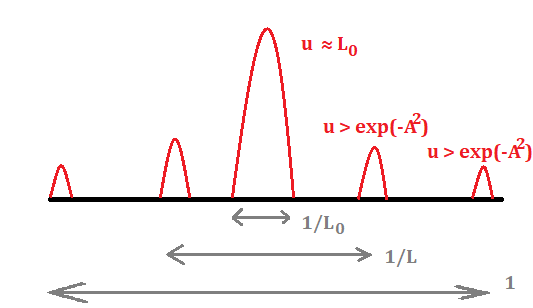
\includegraphics{graphics/heuristic}
		\caption{Concentration of the $L^3_x$-norm at a particular scale implies some uniform amount of concentration of the $L^3_x$-norm at larger scales. In view of the bound on the $L^3_x$-norm, this implies the solution cannot concentrate below a certain length scale. }
	\end{center}
\end{figure}


\begin{theorem}[Non-concentration at high frequencies]
	Let $u: [t_0 - T, t_0] \times \R^3 \to \R^3$ be a classical solution to Navier-Stokes that obeys the a priori $L^\infty_t L^3_x$-bound \eqref{apriori}. Suppose there exists a point in space $x_0 \in \R^3$ and scale $N_0 \in 2^\Z$ which concentrates 
		\begin{equation}
			N^{-1}_0 |P_{N_0} u(t_0, x_0)| \geq A^{-C_0} ,
			\label{eq:concentration}
		\end{equation}
	then
		\begin{equation}
			TN_0^2 \leq \exp \exp \exp A^{O(1)}. \label{eq:exp}
		\end{equation}		
\end{theorem}

Combined with the energy dispersed regularity theorem, this completes the proof of the quantitative regularity theorem. The story of this proof is the (quantitative) contrapositive to the rigidity proof; compare Figures 1 and 3. 

\begin{figure}[h]\label{fig2}
	\begin{center}
		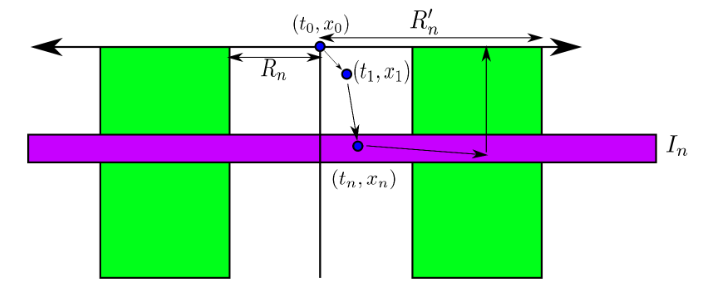
\includegraphics{graphics/stack}
		\caption{Concentration at a point $(t_0, x_0)$ can only hold if there existed previous concentrations in space-time $(t_n, x_n)$. Unique continuation allows one to propagate this concentration on a time-epoch, while backwards uniqueness in a large annulus pushes this concentration back up to the original time $t = t_0$. This can be seen as a lack of compactness of critically bounded solutions. }
	\end{center}
\end{figure}

\subsection{Preliminaries}

Throughout we will use $A \lesssim B$ to denote $A \leq CB$ for some constant $C > 1$, and we will use notation such as $B \approx N$ to denote something like $A^{-O(1)} N \leq B \leq A^{O(1)} N$ and $B \lessapprox N$ to denote something like $B \leq A^{-O(1)} B$, etc. For a more precise picture of how these exponents interact at each step, c.f. Tao. 

\begin{lemma}[General Carleman inequality]\label{lem:carleman}
	Let $w : I \times \R^3 \to \R^3$ be a test function, and denote $L := \partial_t + \Delta$ the backwards heat operator. Then for any weight function $g: I \times \R^3 \to \R$, we have the inequality 
		\[
			\partial_t \int_{\R^3} \left( |\nabla u|^2 + \frac12 F|u|^2 \right) e^g \, dx \geq \int_{\R^3} \left( \frac12 (LF)|u|^2 + 2D^2 g (\nabla u, \nabla u)  - \frac12 |Lu|^2\right) e^g \, dx
		\]
	where	
		\[
			F:= \partial_t g - \Delta g - |\nabla g|^2.
		\]
	In particular, from the fundamental theorem of calculus, one has
		\[
			\int_{t_1}^{t_2} \int_{\R^3} \left( \frac12 (LF) |u|^2 + 2D^2 g(\nabla u, \nabla u) \right) e^g \, dx dt 
				\leq \frac12 \int_{t_1}^{t_2} \int_{\R^3} |Lu|^2 e^g \, dx dt + \left[\int_{\R^3} \left( |\nabla u|^2 + \frac12 F |u|^2\right) e^g \, dx \right]_{t = t_1}^{t = t_2}.
		\]		
\end{lemma}

We will also need a localisation lemma in the spirit of finite speed of propagation for wave equations. More precisely, the Navier-Stokes equations enjoy a finite distance of propagation property, which takes the form of an $L^1_tL^\infty_x$-bound. Heuristically, the energy balance implies control over the dissipation $||\nabla u||_{L^2_{t, x}}$, so dimensional analysis reveals
	\[
		[t]^{1/2} [x]^{1/2} [u] \lesssim 1.
	\]
The non-linear regime is when amplitude is much larger than the frequency scale $[u] \gg [x]^{-1}$, so substituting this into the above we have a bound on a quantity with dimensions
	\[
		[t] [u] \lesssim 1.
	\]

\begin{proposition}[Finite distance of propagation]
	Let $u \in L^\infty_t L^3_x ([0, T] \times \R^3)$ be a classical solution to the Navier-Stokes equations \eqref{NS} satisfying \eqref{apriori}. Then for any interval $I \subseteq [T/2, T]$ we have
		\begin{equation}
			||u||_{L^1_t L^\infty_x (I \times \R^3)} \lessapprox |I|^{1/2}.\label{eq:dist}
		\end{equation}
\end{proposition}

\subsection{Back propagation}

In this section, we show that given a point of concentration \eqref{concentration}, we can find a sequence of points in the backwards parabolic domain of dependence located at approximately  $\log(T N_0^2)$-many scales. This explains the first exponential in the final results. 

\begin{lemma}[Short back propagation] \label{lem:back}
	Let $u: [t_0 - T, t_0] \times \R^3 \to \R^3$ be a classical solution to Navier-Stokes \eqref{NS} that obeys the $L^\infty_t L^3_x$-bound \eqref{apriori}, and suppose there exists a point $(t_i, x_i) \in [t_i - T, t_i] \times \R^3$ and frequency scale $N_1 \in 2^\Z$ at which the solution concentrates
		\[
			N_i^{-1} |P_{N_i} u (t_i, x_i)|
				\geq A^{-C_0},
		\]
	and satisfy
		\begin{align*}
			t_0 - t_i
				&\geq T/2, \\
			N_i
				&\gtrsim T^{-1/2}.	
		\end{align*}	
	Then there exists a previous point in time $(t_{i + 1}, x_{i + 1}) \in [t_0 - T, t_i] \times \R^3$ and frequency scale $N_{i + 1} \in 2^\Z$ at which the solution also concentrates
		\[
			N_{i + 1}^{-1} |P_{N_{i + 1}} u (t_{i + 1}, x_{i + 1})|
				\geq A^{-C_0}
		\]
	and satisfy
		\begin{align*}
			N_{i + 1}
				&\approx N_i,\\
			t_i - t_{i + 1}
				&\approx N_i^{-2},\\
			|x_{i} - x_{i + 1}|
				&\lessapprox N_i^{-1}.
		\end{align*}	
\end{lemma}

\begin{proof}
	Exercise! On a more serious note, this amounts to Littlewood-Paley theory and using Duhamel's formula. If nearby points and neighboring frequencies all don't concentrate, then this concentration could not have happened. This requires some paradifferential calculus which we omit due to laziness. 
\end{proof}


\begin{proposition}[Back propagation to any scales]\label{prop:back}
	Let $u : [t_0 - T, t_0] \times \R^3 \to \R^3$ be a classical solution to Navier-Stokes \eqref{NS} that obeys the $L^\infty_t L^3_x$-bound \eqref{apriori}, and suppose there exists a point $(t_0, x_0) \in [t_0 - T, t_0] \times \R^3$ and frequency scale $N_0 \in 2^\Z$ at which the solution concentrates
		\[
			N_0^{-1} |P_{N_0} u(t_0, x_0)| \geq A^{-C_0}.
		\]
	Then for every time-scale $N_0^{-2} \lessapprox \overline T \lessapprox T$, there exists another point $(\overline t, \overline x) \in [t_0 - \overline T, t_0] \times \R^3$ and frequency scale $\overline N \in 2^\Z$ at which we have concentration
		\[
			{\overline N}^{-1} |P_{\overline N} u(\overline t, \overline x)| \geq A^{-C_0}
		\]
	and satisfy
		\begin{align*}
			t_0 - \overline t
				&\approx \overline T,\\
			\overline N
				&\approx {\overline T}^{-1/2},\\
			|\overline x - x_0|
				&\lessapprox {\overline T}^{1/2}.
		\end{align*}
		
\end{proposition}

\begin{proof}
	Iterating Lemma \ref{lem:back}, we can find a sequence of points $(t_0, x_0), \dots, (t_n, x_n) \in [t_0 - T, t_0] \times \R^3$ and scales $N_1, \dots, N_n \in 2^\Z$ at which the solution concentrates
		\begin{equation}
			N_i^{-1} |P_{N_i} u(t_i, x_i)| \geq A^{-C_0},\label{eq:back}
		\end{equation}
	and satisfying
		\begin{align}
			N_{i + 1}
				&\approx N_i,\label{eq:N}\\
			t_i - t_{i + 1}
				&\approx N_i^{-2},\label{eq:t}\\
			|x_{i} - x_{i + 1}|
				&\lessapprox N_i^{-1}\label{eq:x},
		\end{align}	
	terminating the iteration in finite $n$ when either we reach too far back in time $t_0 - t_n \leq T/2$ or a small enough frequency scale $N_n \lessapprox T^{-1/2}$. Indeed, we can at the very least go back far enough in time using a qualitative argument showing the time separations \eqref{t} are uniformly bounded below. It suffices to show a uniform upper bound on the frequency scales $N_i$; this follows from the concentration inequality \eqref{back} and the \textit{a priori} assumption that $u$ was classical which gives a uniform upper bound on $|P_{N_i} u|$. By construction, the choice of time scale $\overline T$ is between the first and last application of back propagation, 
		\[
			t_n < t_0 - \overline T < t_1.
		\]	
	Consider the last iterate $t_m$ before we pass time scale $\overline T$, i.e. the largest index $m$ such that $t_0 - \overline T \leq t_m$. We want to locate an index $j$ in this range such that the frequency scale is comparable $N_j \approx \overline T^{-1/2}$. By definition of $m$ and telescoping the time separation \eqref{t}, 
		\begin{equation}
			\overline T \leq t_0 - t_{m + 1} \lessapprox \sum_{i = 0}^m N_i^{-2}.\label{eq:l2}
		\end{equation}
	On the other hand, Bernstein, the fundamental theorem of calculus, and \eqref{apriori} allow us to propagate the concentration \eqref{back}, controlling the frequency scale by the speed,
		\[
			||u(t) ||_{L^\infty_x} \gtrsim A^{-C_0} N_i
		\]
	on the interval $t_i - t \lesssim N_i^{-2}$. In view of the time separation \eqref{t}, we can integrate both sides in time on $[t_0 - \overline T, t_0]$, controlling the left-hand side by the distance of propagation estimate \eqref{dist},
		\begin{equation}
			\sum_{i = 0}^m N_i^{-1} \lessapprox \overline T^{1/2}.\label{eq:l1}
		\end{equation}
	Notice that \eqref{l2} is a lower bound on the $\ell^2$-norm of the length scales $N_i^{-1}$, while \eqref{l1} is an upper bound on the $\ell^1$-norm, so interpolating we obtain an estimate for the $\ell^\infty$-norm, i.e. there exists $j = 0, \dots, m$ with
		\[
			N_j^{-1} \approx \overline T^{1/2}.
		\]
	Combined with the estimates on time separation \eqref{t} and spatial separation \eqref{x} and finite distance propagated \eqref{l1}, we can conclude $(t_j, x_j)$ are at the appropriate scale away from the initial point of concentration $(t_0, x_0)$, indeed
		\begin{align*}
			\overline T 
				&\geq t_0 - t_j\\
				&\geq t_{j - 1} - t_j \gtrapprox N_j^{-2} \gtrapprox \overline T, \\
			|x_j - x_0|
				&\leq \sum_{i = 0}^{j - 1} |x_i - x_{i + 1}| \lessapprox \sum_{i = 0}^{j - 1} N_i^{-1} \lessapprox \overline T^{1/2}.	
		\end{align*}
	Taking $\overline N := N_j$ and $(\overline t, \overline x) := (t_j, x_j)$ completes the proof.	
\end{proof}

\begin{figure}[h]
	\begin{center}
		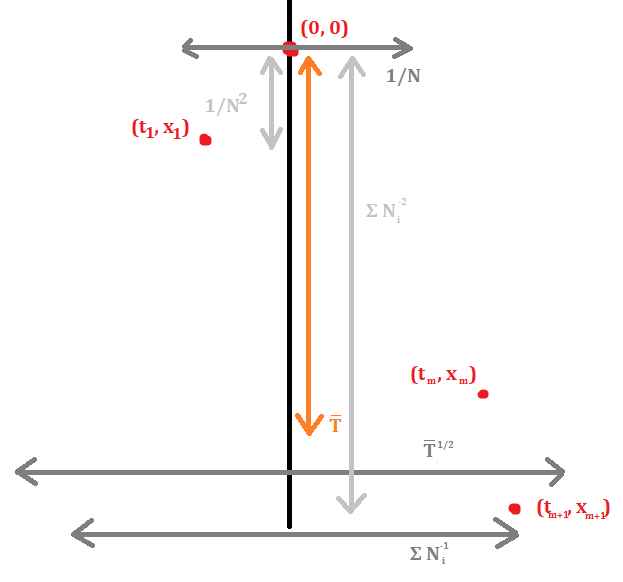
\includegraphics[scale =0.75]{graphics/back}
		\caption{We iterate the short back propagation until we reach the desired time scale. This bounds the time scale $\overline T$ above by the total time separation \eqref{l2}. On the other hand, finite distance of propagation tells us the points could not have traveled too far, bounding the total distance traveled \eqref{l1} by $\overline T^{1/2}$. Thus one of the spatial separations must have been large $N^{-1}_j \gtrsim \overline T^{1/2}$.}
	\end{center}
\end{figure}

\begin{remark}
	Note that we used the \textit{qualitative} fact that $u$ was a classical solution in order to guarantee that the iteration reaches far back enough in time. This is pretty funny...
\end{remark}



\subsection{Unique continuation in epochs of regularity}

Now that we have located points of concentration at different scales, we want to propagate this concentration sufficiently far in space so as to intersect an annuli of regularity in the following subsection. This will follow from unique continuation applied to the vorticity equation \eqref{vortNS}, provided we obtain pointwise bounds for the coefficients $u$ and $\nabla u$. The Carleman estimates we use here gain us another exponential in our estimates. 

\begin{proposition}[Epochs of regularity]\label{prop:epoch}
	Let $u : [t_0 - T, t_0] \times \R^3 \to \R^3$ be a classical solution to Navier-Stokes \eqref{NS}  that obeys the a priori $L^\infty_t L^3_x$-bound \eqref{apriori}. Then for any interval $I \subseteq [t_0 - T/2, t_0]$, there exists a sub-interval $J \subseteq I$ with comparable size $|J| \approx |I|$ on which the solution is regular
		\[
			||\nabla^j u ||_{L^\infty_{t, x} (J \times \R^3)} \lessapprox |I|^{-\frac{j + 1}{2}}.
		\]
\end{proposition}

\begin{proof}
	By scaling and translation, we can work on $[0, 2]$ and prove the result for the interval $I = [1, 2]$. We split the velocity field into the linear component $u^\lin := e^{t \Delta} u_0$ and non-linear component $u = u^\lin + u^\nlin$.	We argue by the energy method, defining the enstrophy-type quantity
		\[
			E(t)
				:= \frac12 \int_{\R^3} |\nabla u^\nlin |^2 \, dx.
		\]
	By the usual multiplier argument applied to the equation for $\nabla u^\nlin$, we can write
		\[
			\partial_t E(t)
				= - \int_{\R^3} |\nabla^2 u^\nlin|^2 \, dx + \int_{\R^3} \Delta u^\nlin \cdot (\nabla \cdot (u \otimes u))\, dx.
 		\]
 	To conclude, we aim for control over the sub-critical quantities $E(t)$ and $||\nabla^2 u^\nlin||_{L^2_{t, x}}$ on a sub-interval of length $|J| \approx 1$. To control the non-linear term on the right, we use Holder's inequality to place the linear components of $u \otimes u$ into a higher $L^p$-space to apply parabolic smoothing, and Sobolev inequalities to handle the non-linear components, 
 		 \begin{align*}
 			||\nabla \cdot (u \otimes u)||_{L^2_x}
 					&\lesssim ||u||_{L^6_x} ||\nabla u||_{L^3_x}\\
 					&\lesssim (A + ||u^\nlin||_{L^6_x} ) (A + ||\nabla u^\nlin ||_{L^3_x}) \\
 					&\lesssim (A + E(t)^{1/2} ) (A +E(t)^{1/4} ||\nabla^2 u^\nlin||_{L^2_x}^{1/2}).
 		\end{align*}
 	Using Young's inequality, we can peel off the dissipation terms $\nabla^2 u^\nlin$ to conclude
 		\begin{align*}
 			\partial_t E(t)
 				&\leq - \frac12 ||\nabla^2 u^\nlin||_{L^2_x}^2 + \frac12 ||\nabla \cdot (u \otimes u)||_{L^2_x}^2\\
 				&\leq - \frac14||\nabla^2 u^\nlin||_{L^2_x}^2  + O(A^4 + A^4 E(t) + E(t)^3).
 		\end{align*}
 	We know that 
 		\[
 			\int_1^2 E(t) \, dt \lesssim A^4.
 		\]
 	Thus, by the pigeonhole principle, there exists a time $t_0 \in [1, 1/2]$ such that 
 		\[
 			E(t_0) \lesssim A^4.
 		\]	
 	A standard continuity argument allows us to extend the inequality above for $t - t_0 \lesssim cA^{-8}$. Putting this back into the energy estimate also controls the enstrophy dissipation on this interval, 
 		\[
 			\int_J \int_{\R^3} |\nabla^2 u^\nlin|^2 \, dx dt \lesssim A^4.
 		\]
 	This gives enough sub-critical control to close the argument. 	
\end{proof}


\begin{proposition}[Unique continuation]
	Let $w : [0, T] \times \R^3 \to \R^3$ be a smooth function obeying the differential inequality 
		\[
			|Lw| \leq C_0^{-1} T^{-1} |u| + C_0^{-1/2}T^{-1/2} |\nabla u|
		\]
	on a space-time cylinder $t \in [0, T]$ and $|x| \leq r$ of sufficiently large radius $r^2 \geq 4000 T$. Then $w$ obeys for any $0 < t_1 \leq t_0 < T/1000$ the Carleman estimate
		\[
			\int_{t_0}^{2t_0} \int_{|x| \leq r/2} (T^{-1} |w|^2 + |\nabla w|^2) e^{-|x|^2/4t} \, dx dt \lesssim e^{-r^2/500t_0} X + t_0^{3/2} (et_0/t_1)^{O(r^2/t_0)} Y,
		\]	
	where
		\begin{align*}
			X
				&:= \int_0^T \int_{|x| \leq r} (T^{-1} |w|^2 + |\nabla v|^2) \, dx dt, \\
			Y
				&:= \int_{|x| \leq r} |w(0)|^2 t_1^{-3/2} e^{-|x|^2/4t_1} \, dx.	
		\end{align*}	
\end{proposition}

\begin{proof}
	Plug in the weight
		\[
			g:= - \frac{|x|^2}{4(t + t_1)} - \frac32 \log (t + t_1) - \alpha \log \frac{t + t_1}{T_0 + t_1} + \alpha \frac{t + t_1}{T_0 + t_1}.
		\]
	into Lemma \ref{lem:carleman}. 	
\end{proof}

\begin{remark}
	The estimate tells us that $w$ and $\nabla w$ are controlled in a weighted $L^2_{t, x}$-sense by the same quantity on a larger region with a gain in decay of $e^{-r^2/500t_0}$ and the contribution of the $L^2_x$-norm near the origin at the initial time. If $w$ vanishes to infinite order at the origin, sending $t_1, t_0 \to 0$ the right-hand side vanishes, so $w\equiv 0$ everywhere, up to making sense of the left-hand side. Compare with Proposition \ref{prop:unique1}. 
\end{remark}	

Armed with the epoch of regularity and unique continuation, let us propagate the concentration into any sufficiently large annuli in space. Suppose we started, without loss of generality, with concentration at the origin $(t_0, x_0) = (0, 0)$ at scale $N_0 \in 2^\Z$, then given any given a time-scale $N_0^{-2}\lessapprox \overline T \lessapprox T$, we can find a point of concentration $(\overline t, \overline x)$ at scales
		\begin{align*}
			 - \overline t
				&\approx \overline T,\\
			\overline N
				&\approx {\overline T}^{-1/2},\\
			|\overline x|
				&\lessapprox {\overline T}^{1/2}.
		\end{align*}
Up to lower order error terms and possibly shifting slightly in space, $P_{\overline N} \omega \sim P_{\overline N} \nabla u \sim \overline N P_{\overline N} u$, and we also have the derivative bounds $\nabla P_{\overline N} \omega = O(A \overline N^3)$ and $\partial_t P_{\overline N} \omega = O(A \overline N^4)$, so the vorticity is also concentrated
	\[
		|P_{\overline N} \omega (t, x)| \gtrsim A^{-C_0} \overline N^2
	\]
in a space-time region of size $t - t_1 \approx \overline N^{-2}$ and $|x - \overline x| \approx \overline N^{-1}$. We now locate an epoch of regularity in this time slice $|J| \approx \overline T$ on which we have good pointwise bounds in $J \times \R^3$ for both $u$ and $\omega$, 
	\begin{align*}
		|\nabla^j u|
			&\lessapprox \overline T^{-\frac{j + 1}{2}}, \\
		|\nabla^j \omega|
			&\lessapprox \overline T^{-\frac{j + 2}{2}}.
	\end{align*}
We can always shrink the epoch of regularity so that the bounds on the coefficients $\nabla^j u$ in the vorticity equation imply that the differential inequality is satisfied. Write $J = [t' - T', t']$ and let $x_* \in \R^3$ be any point far away $|x_*| \gtrapprox \overline T^{1/2}$. Applying unique continution on $J$ with radius $r = A^{O(1)} |x_*|$ and $t_0 = T'/2$ and $t_1 = A^{-O(1)}T'$, we have
	\[
		Z \lesssim \exp (-A^{O(1)} |x_*|^2 / T') X + |T'|^{3/2} \exp(A^{O(1)} |x_*|^2/T') Y
	\]
where
	\begin{align*}
		X
			&:= \int_{J} \int_{B_{A^{O(1)} |x_*|} (x_*) } (|T'|^{-1} |\omega|^2 + |\nabla \omega|^2) \, dx dt,\\
		Y
			&:= |T'|^{-3/2} \int_{B_{A^{O(1)}|x_*|}  (x_*)} |\omega(t')|^2 e^{-A^{O(1)} |x - x_*|^2/4T'} \, dx,\\
		Z
			&:=\int_{t' - T'}^{t' - T'/2} \int_{B_{A^{O(1)}|x_*|/2}  (x_*)}	 |T'|^{-1} |\omega|^2 e^{-|x - x_*|^2/4(t' - t)} dx dt.
	\end{align*}	
Observe $Z$ is bounded below, using the trivial lower bound on the heat kernel, and concentration of $\omega$, 
	\[
		Z \gtrsim A^{-O(1)} \exp(-|x_*|^2/100T') |T'|^{-1/2}
	\]
On the other hand, the good bounds on $\omega$ in the epoch of regularity and the gain of $\exp(-A^{O(1)} |x_*|^2/T')$ on the right tells us that the contribution of $X$ is negligible compare to the lower bound on $Z$. This furnishes a lower bound for $Y$. The weights in the $Y$ integral and the good bounds on $\omega$ tell us that the contribution in the region $|x_* - x| >|x_*|/2$ are negligible, so the lower bound on $Y$ implies
	\[
		\int_{B_{|x_*|/2} (x_*)} |\omega(t')|^2 \, dx \gtrsim \exp (-A^{O(1)} |x_*|^2/T') |T'|^{-1/2}. 
	\]
This ball is located in a large annulus, and integrating over the time interval $J$, we conclude the bound
	\[
		\int_{-\overline T}^{-A^{-O(1)} \overline T} \int_{R/2 \leq |x| \leq 2R} |\omega|^2 \, dx dt \gtrsim \exp (-A^{O(1)} R^2/\overline T) \overline T^{1/2}
	\]
for any time scale $\overline T$ and spatial scale $R$ satisfying $N_0^{-2} \lessapprox \overline T \lessapprox T$ and $R \gtrapprox \overline T^{1/2}$. 

\subsection{Backwards uniqueness on annuli of regularity}

It remains to show that these concentrations in large annuli far back in time imply concentration in the annuli at the original time of concentration. As in the previous section, we rely on Carleman estimates, however we cannot exploit the size of the interval to get good bounds on the coefficients of the vorticity equation. Instead, we rely on a dyadic pigeonholing argument to find large annuli where the enstrophy is small, and bounded total speed to show that this persists up until the original time up to shrinking our annuli. This dyadic pigeonholing argument is the source of the final exponential in the conclusion. 

\begin{figure}[h]
	\begin{center}
		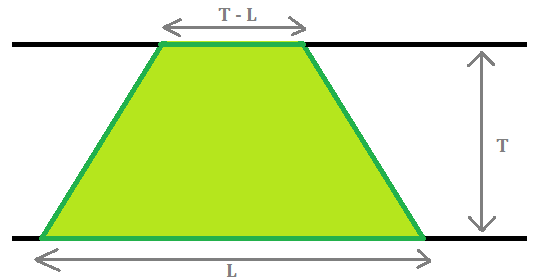
\includegraphics[scale = 0.8]{graphics/finite}
		\caption{For wave equations, we can use finite speed of propagation to localise regularity. More precisely, if a solution is smooth in a ball, it is smooth in the domain of dependence. A similar result holds for Navier-Stokes using \eqref{dist} allowing us to localise the enstrophy estimates.}
	\end{center}
\end{figure}


\begin{proposition}[Annuli of regularity]
	Let $u : [t_0 - T, t_0] \times \R^3 \to \R^3$ be a classical solution to Navier-Stokes \eqref{NS}  that obeys the a priori $L^\infty_t L^3_x$-bound \eqref{apriori}. Then for every time-scale $0 < \overline T < T/2$ and large radius $R_0 \geq \overline T ^{1/2}$, there exists an annulus 
	\[
			\Omega 
				:= \{ (t, x) \in [t_0 - \overline T, t_0] \times \R^3 :  R \leq |x - x_0| \lessapprox A_6 R\},
	\]
	at scale
	\[
			 R_0 \leq R \leq \exp (A^{O(1)}) R_0,
	\]
	on which 	 
		\[
			||\nabla^j u ||_{L^\infty_{t, x} (\Omega)}\ll \overline T^{- \frac{j + 1}{2}}.
		\]	
\end{proposition}

\begin{proof}
	By scaling and translation, we can work on $[0, 2]$, and prove the result for $\overline T = 1$. We split the velocity and vorticity fields into the linear components, $u^\lin := e^{t \Delta} u_0$ and $\omega^\lin := e^{t \Delta} \omega_0$, and non-linear components, $u = u^\lin + u^\nlin$ and $\omega = \omega^\lin + \omega^\nlin$. We have an a priori estimate on 
		\[
			\int_{1/2}^2  \int_{\R^3} |\nabla u^\nlin |^2 \, dx dt \lesssim A^4.
		\]
	Pigeonholing, we can find $1/2 \leq t_1 \leq \overline T$ such that 	
		\[
			\int_{\R^3}  |\nabla u^\nlin (t_1)|^2 \, dx  \lesssim A^4. 
		\]
	We want to propagate enstrophy bounds up to time $t = 1$, and, since we no longer have smallness of time interval, we need this control to be very small. To do this, we use a dyadic pigeonholing argument, which implies that there exists a scale 
		\[
			A^{O(1)} R_0 \leq R \leq \exp(A^{O(1)}) R_0
		\]
	such that 
		\[
			\int_{|x| \approx R} |\nabla u^\nlin (t_1)|^2 \lesssim A^{-O(1)}. 
		\]	
	Let $R_- \ll R$ and $R_+ \gg R$ to be chosen later, set	
		\begin{align*}
			R_- (t)
				&:= R_- + C_0 \int_{t_1}^t ( A^{O(1)} + ||u (s)||_{L^\infty_x}) \, ds \\
			R_+ (t)
				&:= R_+ - C_0 \int_{t_1}^t ( A^{O(1)} + ||u (s)||_{L^\infty_x}) \, ds	
		\end{align*}
	We argue by the energy method, defining the enstrophy as localised to the annuli where we expect regularity to persist in time. Set
		\[
			\eta(t, x) := \max \left( \min(A^{O(1)} , |x| - R_- (t), R_+ (t) - |x|) , 0  \right).
		\]
	By construction, $\eta$ is supported in $R_- \leq |x| \leq R_+$, has Lipschitz norm $1$, and is constant $\eta \equiv A^{O(1)}$ in the smaller annulus $R_- + A^{O(1)} \leq |x| \leq R_+ - A^{O(1)}$. Define the local enstrophy
		\[
			E(t)
				:= \frac12 \int_{\R^3} |\omega^\nlin|^2 \eta \, dx.
		\]
	This is small at time $t_1$. We need to control the time derivative to propagate this smallness. We compute
		\[
			\partial_t E(t) = -Y_1 (t) - Y_2 (t) + Y_3 (t) + Y_4 (t) + Y_5 (t) + Y_6 (t) + Y_7 (t) + Y_8 (t) + Y_9 (t),
		\]
	where $Y_1$ is the dissipation, $Y_2$ is the recession, $Y_3$ is the heat flux, $Y_4$ is the transport term, $Y_5, Y_7, Y_8, Y_9$ are corrections to transport, $Y_6$ is the main non-linear term
		\begin{align*}
			Y_1 (t)
				&:= \int_{\R^3} |\nabla \omega^\nlin |^2 \, dx,\\
			Y_2 (t)
				&:= -\frac12 \int_{\R^3} |\omega^\nlin |^2 \partial_t \eta \, dx, \\
			Y_3 (t)
				&:= \frac12 \int_{\R^3} |\omega^\nlin|^2 \Delta \eta \, dx, \\
			Y_4 (t)
				&:= \frac12 \int_{\R^3} |\omega^\nlin|^2 u \cdot \nabla \eta \, dx, \\
			Y_6 (t)
				&:= \int_{\R^3} \omega^\nlin \cdot (\omega^\nlin \cdot \nabla) u^\nlin \, \eta \, dx. 				
		\end{align*}
	We aim to control $Y_3, \dots, Y_9$ in terms of $Y_1, Y_2, E$. Observe that 
		\[
			-\partial_t \eta = C_0 (A^{O(1) }+ ||u||_{L^\infty_x}) |\nabla \eta|,
		\]
	so $Y_2$ has good sign. The worst term is like $\int |\omega^\nlin|^3 \, \eta$, with the caveat that $\nabla u^\nlin \approx \omega^\nlin$ is a caricature which doesn't capture the non-local nature of the Biot-Savart law. We estimate
		\begin{align*}
			Y_6 (t)
				\lesssim  \int_{\R^3} |\omega^\nlin|^3 \, dx 
				\lesssim Y_1 + E(t)^{1/2} Y_1 + A^{-O(1)} + E(t)^2 Y_1
		\end{align*}
	Collecting our estimates, 
		\[
			\partial_t E(t) 
				\leq - \frac12 Y_1 (t) + O\left(E(t) + |Y_3 (t)| + |Y_{10} (t)| + A_6^{-1} + E(t)^{1/2} Y_1 (t) + E(t)^2 Y_1 (t) \right)
		\]	
	Then 
		\begin{align*}
			E(t)
				&\lessapprox 1, \\
			\int_{t_1}^1 Y_1 (t) \, dt
				&\lessapprox 1. 	
		\end{align*}	
	This is enough sub-critical control to close the argument. (ADD MORE DETAILS: WHITNEY DECOMPOSITION SEEMS NECESSARY TO HANDLE CUTOFF) 	
\end{proof}


\begin{proposition}[Backwards uniqueness]
	Let $w : [0, T] \times \R^3 \to \R^3$ be a smooth function obeying the differential inequality 
		\[
			|Lw| \leq C_0^{-1} T^{-1} |w| + C_0^{-1/2} T^{-1/2} |\nabla w|
		\]
	on the annulus $t \in [0, T]$ and $r_- \leq |x| \leq r_+$ which is sufficiently far out $r_-^2 \geq 4C_0 T$. Then $w$ obeys the Carleman estimate
		\[
			\int_0^{T/4} \int_{10 r_- \leq |x| \leq r_+/2}T^{-1} |u|^2 + |\nabla u|^2 \, dx dt
				\lesssim C_0^2 e^{-r_-r_+/4C_0 T} (X + e^{2r^2_+/C_0T} Y),
		\]	
	where
		\begin{align*}
			X
				&:= \int_0^T \int_{r_- \leq |x| \leq r_+} e^{2|x|^2/C_0 T} (T^{-1} |w|^2 + |\nabla w|^2) \, dx dt, \\
			Y
				&:= \int_{r_- \leq |x| \leq r_+} |w(0)|^2 \, dx.
		\end{align*}	
\end{proposition}	

\begin{proof}
	Apply the weight
		\[
			g:= \alpha (T_0 - t) |x| + \frac{1}{C_0 T} |x|^2
		\]
	in the Carleman inequality, Lemma \ref{lem:carleman}. The general idea is convexity of $g$ so that $D^2 g$ is coercive, and apply a cut-off to the region of interest.
\end{proof}

\begin{remark}
	The estimate tells us that $w$ and $\nabla w$ are controlled in $L^2_{t, x}$-norm on an annulus by itself in a larger annulus with a weight, but also a gain in decay $e^{-r_- r_+/4C_0 T}$ which is favourable when the ratio of radii is large $r_+/r_- \gg 1$, and also the $L^2$-norm at the initial time with a large weight. Assuming $w$ vanishes at the initial time, taking $r_+ \to \infty$ implies it vanishes in space-time. Compare with Proposition \ref{prop:backunique1}.
\end{remark}

Let us return to where we left off in the previous subsection and finish off the proof of the theorem. We showed that for any time-scale $N_0^{-2} \lessapprox \overline T \lessapprox T$, there is $L^2_{t, x}$-concentration on every annulus with sufficiently large radius $R \gtrapprox \overline T^{1/2}$, namely
\[
		\int_{-\overline T}^{-A^{-O(1)} \overline T} \int_{R/2 \leq |x| \leq 2R} |\omega|^2 \, dx dt \gtrsim \exp (-A^{O(1)} R^2/\overline T) \overline T^{1/2}.
	\]
In this range of scales, we can choose an annulus of regularity $\overline T^{1/2} \lessapprox R \lessapprox \exp(A^{O(1)}) \overline T^{1/2}$ on which we have small pointwise bounds on $u$ and $\omega$ for all time $t \in [0, T]$, 
	\begin{align*}
		|\nabla^j u|
			&\ll \overline T^{-\frac{j + 1}{2}}, \\
		|\nabla^j \omega |
			&\ll \overline T^{-\frac{j + 2}{2}}	.
	\end{align*}
This allows us to apply backwards uniqueness on $[0, \overline T/C_0]$ with $r_- = 10R$ and $r_+ = A^{O(1)} R/10$, giving
	\[
		Z \lesssim \exp (-A^{O(1)} R^2/ \overline T) X + \exp (\exp (A^{O(1)})) Y
	\]
where
	\begin{align*}
		X
			&:= \int_{-\overline T/C_0}^0  \int_{10 R \leq |x| \leq A^{O(1)} R/10} e^{2|x|^2/\overline T} (\overline T^{-1} |\omega| + |\nabla \omega|^2) \, dx dt, \\
		Y
			&:= \int_{10 R \leq |x| \leq A^{O(1)} R/10} |\omega(0)|^2 \, dx ,\\
		Z
			&:= \int_{-\overline T/4C_0}^0 \int_{100 R \leq |x| \leq A^{C_0} R/20} \overline T^{-1} |\omega|^2 \, dx dt.
	\end{align*}
We have a lower bound for $Z$ coming from the previous unique continuation argument, so either $X$ or $Y$ sees the concentration. If $Y$ sees the concentration, then we are in good shape, since we get an estimate of the form 
	\[
		\int_{2R \leq |x| \leq A^{O(1)} R/2} |\omega(0)|^2 \, dx \gtrsim \exp (- \exp (A^{O(1)}) ) \overline T^{-1/2}.
	\]
We unfortunately cannot treat $X$ as negligible since the size of the gain in decay is comparable to the size of concentration. However, we can extract a small ball inside this annulus of concentration and run the unique continuation argument, this time with $Y$ measuring the norm at time $t = 0$ since we are in an annulus of regularity. Thus we obtain the bound above regardless. We would like to use this to show the $L^3_x$-norm of $u$ concentrates. The annulus has volume $O(\exp (\exp (A^{O(1)})) \overline T^{3/2})$ so pigeonholing we can find a point of concentration in this annulus
	\[
		|\omega(0, x_*)| \gtrsim  \exp (- \exp (A^{O(1)}) ) \overline T^{-1}.
	\]
We can propagate this in space since $|\nabla \omega |
\ll \overline T^{-\frac{3}{2}}$, while integration-by-parts against a cut-off and Holder's inequality gives us a lower bound on the $L^3_x$-norm in a ball of radius $r = \exp(-\exp(A^{O(1)})) \overline T^{1/2}$, which is in turn contained by the annulus, 
	\[
		\int_{\overline T^{1/2} \leq |x| \lessapprox \overline T^{1/2}} \geq \int_{B_r (x_*)} |u(t_0)|^3 \, dx \gtrsim \exp (-\exp(A^{O(1)})).
	\]
Summing over disjoint scales,
	\[
		\int_{\R^3} |u(t_0)|^3 \, dx \gtrsim  \exp (-\exp(A^{O(1)}))\log(TN_0^2),
	\]
this completes the proof. 	


\bibliographystyle{alpha}
\bibliography{external/biblio}

\end{document}
